\documentclass[12pt,twoside]{article}

%% Gebaseerd op
% Leerplan 2006-059
% Ruimtemeetkunde deel I, Lineaire Algebra van Liliane Van Maldeghem en Hendrik Van Maldeghem
% Wiskundige Basisvaardigheden van Gert Sonck, Wolfgang Jacquet en Tom Dorissen


\textwidth 17cm \textheight 25cm \evensidemargin 0cm
\oddsidemargin 0cm \topmargin -2cm
\parindent 0pt
%\parskip \bigskipamount

\usepackage{graphicx}
\usepackage[dutch]{babel}
\usepackage{amssymb,amsthm,amsmath}
%\usepackage{dot2texi}
\usepackage[utf8]{inputenc}
\usepackage{nopageno}
\usepackage{pdfpages}
\usepackage{enumerate}
\usepackage{caption}
\usepackage{wrapfig}
\usepackage{pgf,tikz,pgfplots}
\pgfplotsset{compat=1.15}
\usepackage{color}
\usetikzlibrary{arrows}
\usetikzlibrary{patterns}
\usepackage{fancyhdr}
\pagestyle{fancy}
\usepackage[version=3]{mhchem}
\usepackage{multicol}
\usepackage{fix-cm}
\usepackage{setspace}
\usepackage{mhchem}
\usepackage{xhfill}
\usepackage{parskip}
\usepackage{cancel}
\usepackage{mdframed}
\usepackage{url}
\usepackage{mathtools}
\usepackage{changepage}

\newcommand{\todo}[1]{{\color{red} TODO: #1}}

\newcommand{\degree}{\ensuremath{^\circ}}
\newcommand\rad{\qopname\relax o{\mathrm{rad}}}

\newcommand\ggd{\qopname\relax o{\mathrm{ggd}}}

\pgfmathdeclarefunction{gauss}{2}{%
  \pgfmathparse{1/(#2*sqrt(2*pi))*exp(-((x-#1)^2)/(2*#2^2))}%
}

\def\LRA{\Leftrightarrow}

\newcommand{\zrmbox}{\framebox{\phantom{EXE}}\phantom{X}}
\newcommand{\zrm}[1]{\framebox{#1}}

% environment oefening:
% houdt een teller bij die de oefeningen nummert, probeert ook de oefening op één pagina te houden
\newcounter{noefening}
\setcounter{noefening}{0}
\newenvironment{oefening}
{
  \stepcounter{noefening}
  \pagebreak[0]
  \begin{minipage}{\textwidth}
  \vspace*{0.7cm}{\large\bf Oefening \arabic{noefening}}
}{%
  \end{minipage}
}

\usepackage{calc}

% vraag
\reversemarginpar
\newcounter{punten}
\setcounter{punten}{0}
\newcounter{nvraag}
\setcounter{nvraag}{1}
\newlength{\puntwidth}
\newlength{\boxwidth}
\newcommand{\vraag}[1]{
\settowidth{\puntwidth}{\Large{#1}}
\setlength{\boxwidth}{1.5cm}
\addtolength{\boxwidth}{-\puntwidth}
{\large\bf Vraag \arabic{nvraag} \addtocounter{nvraag}{1}}\vspace*{-0.5cm}
{\marginpar{\color{lightgray}\fbox{\parbox{1.5cm}{\vspace*{1cm}\hspace*{\boxwidth}{\Large{#1}}}}}
\vspace*{0.5cm}}
\addtocounter{punten}{#1}}

% arulefill
\def\arulefill{\leavevmode{\xrfill[-5pt]{0.3pt}[lightgray]\endgraf}\vspace*{0.2cm}}

% \arules{n}
\newcommand{\arules}[1]{
\color{lightgray}
%\vspace*{0.05cm}
\foreach \n in {1,...,#1}{
  \vspace*{0.75cm}
  \hrule height 0.3pt\hfill
}\color{black}\vspace*{0.2cm}}

% \arule{x}
\newcommand{\arule}[1]{
\color{lightgray}{\raisebox{-0.1cm}{\rule[-0.05cm]{#1}{0.3pt}}}\color{black}
}

% \abox{y}
\newcommand{\abox}[1]{
\fbox{
\begin{minipage}{\textwidth- 4\fboxsep}
\hspace*{\textwidth}\vspace{#1}
\end{minipage}
}
}

\newcommand{\ruitjes}[1]{
\definecolor{cqcqcq}{rgb}{0.85,0.85,0.85}
\hspace*{-2.5cm}
\begin{tikzpicture}[scale=1.04,line cap=round,line join=round,>=triangle 45,x=1.0cm,y=1.0cm]
\draw [color=cqcqcq, xstep=0.5cm, ystep=0.5cm] (0,-#1) grid (20.5,0);
\end{tikzpicture}
}


\newcommand{\assenstelsel}[5][1]{
\definecolor{cqcqcq}{rgb}{0.65,0.65,0.65}
\begin{tikzpicture}[line cap=round,line join=round,>=triangle 45,x=#1cm,y=#1cm]
\draw [color=cqcqcq,dash pattern=on 1pt off 1pt, xstep=1.0cm,ystep=1.0cm] (#2,#4) grid (#3,#5);
\draw[->,color=black] (#2,0) -- (#3,0);
%\draw[shift={(1,0)},color=black] (0pt,2pt) -- (0pt,-2pt) node[below] {\footnotesize $1$};
%\draw[color=black] (#3.25,0.07) node [anchor=south west] {$x$};
\draw[->,color=black] (0,#4) -- (0,#5);
%\draw[shift={(0,1)},color=black] (2pt,0pt) -- (-2pt,0pt) node[left] {\footnotesize $1$};
\draw[color=black] (0.09,#5.25) node [anchor=west] {\phantom{$y$}};
%\draw[color=black] (0pt,-10pt) node[right] {\footnotesize $0$};
\end{tikzpicture}
}

\newcommand{\getallenas}[3][1]{
\definecolor{cqcqcq}{rgb}{0.65,0.65,0.65}
\begin{tikzpicture}[scale=#1,line cap=round,line join=round,>=triangle 45,x=1.0cm,y=1.0cm]
\draw [color=cqcqcq,dash pattern=on 1pt off 1pt, xstep=1.0cm,ystep=1.0cm] (#2,-0.2) grid (#3,0.2);
\draw[->,color=black] (#2.25,0) -- (#3.5,0);
\draw[shift={(0,0)},color=black] (0pt,2pt) -- (0pt,-2pt) node[below] {\footnotesize $0$};
\draw[shift={(1,0)},color=black] (0pt,2pt) -- (0pt,-2pt) node[below] {\footnotesize $1$};
\draw[color=black] (#3.25,0.07) node [anchor=south west] {$\mathbb{R}$};
\end{tikzpicture}
}

\newcommand{\visgraad}[1]{\begin{tabular}{p{0.5cm}|p{#1}}&\\\hline\\\end{tabular}}

\newcommand{\tekenschema}[2]{\begin{tabular}{p{0.5cm}|p{#1}}&\\\hline\\[#2]\end{tabular}}

% schema van Horner
\newcommand{\schemahorner}{
\begin{tabular}{p{0.5cm}|p{7cm}}
&\\[1.5cm]
\hline\\
\end{tabular}}

% geef tabular iets meer ruimte
\setlength{\tabcolsep}{14pt}
\renewcommand{\arraystretch}{1.5}

\newcommand{\toets}[3]{
\thispagestyle{plain}
\vspace*{-2.5cm}
\begin{tikzpicture}[remember picture, overlay]
    \node [shift={(15.25 cm,-1.6cm)}] {%
        \includegraphics[width=1.8cm]{/home/ppareit/kaa1415/logokaavelgem.png}%
    };%
\end{tikzpicture}

\begin{tabular}{|llc|c|}
\hline
\vspace*{-0.5cm}
&&&\\
Naam & \arule{4cm} & {\Large\bf KA AVELGEM} & \\
\vspace*{-0.75cm}
&&&\\
Klas & \arule{4cm} & {\Large\bf 20...-...-...} & \\
\hline
\vspace*{-0.75cm}
&&&\\
Toets & {\bf #2} & {\large\bf #1} & Beoordeling\\
\vspace*{-0.75cm}
&&&\\
Onderwerp & \multicolumn{2}{l|}{\bf #3} &\\
\hline
\end{tabular}
}

\newcommand{\oefeningen}[1]{

\fancyhead[LE, RO]{\vspace{0.5cm} #1}
%\thispagestyle{plain}

{\bf \Large \centering Oefeningen: #1}

}

\raggedbottom

\newcommand\vl{\qopname\relax o{\mathrm{vl}}}

\newcommand\dom{\qopname\relax o{\mathrm{dom}}}
\newcommand\ber{\qopname\relax o{\mathrm{ber}}}

\newcommand\mC{\qopname\relax o{\mathrm{mC}}}
\newcommand\uC{\qopname\relax o{\mathrm{{\mu}C}}}
\newcommand\C{\qopname\relax o{\mathrm{C}}}

\newcommand\W{\qopname\relax o{\mathrm{W}}}
\newcommand\kW{\qopname\relax o{\mathrm{kW}}}
\newcommand\kWh{\qopname\relax o{\mathrm{kWh}}}


\newcommand\V{\qopname\relax o{\mathrm{V}}}
\newcommand\ohm{\qopname\relax o{\mathrm{\Omega}}}
\newcommand\kohm{\qopname\relax o{\mathrm{k\Omega}}}


\newcommand\N{\qopname\relax o{\mathrm{N}}}

\newcommand\Nperkg{\qopname\relax o{\mathrm{N/kg}}}

\newcommand\Nperm{\qopname\relax o{\mathrm{N/m}}}

\newcommand\gpermol{\qopname\relax o{\mathrm{g/mol}}}


\newcommand\kgperm{\qopname\relax o{\mathrm{kg/m}}}
\newcommand\kgperdm{\qopname\relax o{\mathrm{kg/dm}}}
\newcommand\gpercm{\qopname\relax o{\mathrm{g/cm}}}
\newcommand\gperml{\qopname\relax o{\mathrm{g/ml}}}


\newcommand{\mA}{\;\mbox{mA}}
\newcommand{\A}{\;\mbox{A}}
\newcommand{\MA}{\;\mbox{MA}}

\newcommand{\us}{\;\mu\mbox{s}}
\newcommand\s{\qopname\relax o{\mathrm{s}}}

\newcommand\h{\qopname\relax o{\mathrm{h}}}

\newcommand{\kmperh}{\;\mbox{km/h}}
\newcommand{\mpers}{\;\mbox{m/s}}
\newcommand{\kmpermin}{\;\mbox{km/min}}
\newcommand{\kmpers}{\;\mbox{km/s}}

\newcommand{\mph}{\;\mbox{mph}}

\newcommand{\Hz}{\;\mbox{Hz}}

\newcommand\Gm{\qopname\relax o{\mathrm{Gm}}}
\newcommand\Mm{\qopname\relax o{\mathrm{Mm}}}
\newcommand\km{\qopname\relax o{\mathrm{km}}}
\newcommand\hm{\qopname\relax o{\mathrm{hm}}}
\newcommand\dam{\qopname\relax o{\mathrm{dam}}}
\newcommand\m{\qopname\relax o{\mathrm{m}}}
\newcommand\dm{\qopname\relax o{\mathrm{dm}}}
\newcommand\cm{\qopname\relax o{\mathrm{cm}}}
\newcommand\mm{\qopname\relax o{\mathrm{mm}}}
\newcommand\um{\qopname\relax o{\mathrm{{\mu}m}}}
\newcommand\nm{\qopname\relax o{\mathrm{nm}}}


\newcommand\Gg{\qopname\relax o{\mathrm{Gg}}}
\newcommand\Mg{\qopname\relax o{\mathrm{Mg}}}
\newcommand\kg{\qopname\relax o{\mathrm{kg}}}
\newcommand\hg{\qopname\relax o{\mathrm{hg}}}
\renewcommand\dag{\qopname\relax o{\mathrm{dag}}}
\newcommand\g{\qopname\relax o{\mathrm{g}}}
\newcommand\dg{\qopname\relax o{\mathrm{dg}}}
\newcommand\cg{\qopname\relax o{\mathrm{cg}}}
\newcommand\mg{\qopname\relax o{\mathrm{mg}}}
\newcommand\ug{\qopname\relax o{\mathrm{{\mu}g}}}
\renewcommand\ng{\qopname\relax o{\mathrm{ng}}}

\newcommand\ton{\qopname\relax o{\mathrm{ton}}}

\newcommand\Gl{\qopname\relax o{\mathrm{Gl}}}
\newcommand\Ml{\qopname\relax o{\mathrm{Ml}}}
\newcommand\kl{\qopname\relax o{\mathrm{kl}}}
\newcommand\hl{\qopname\relax o{\mathrm{hl}}}
\newcommand\dal{\qopname\relax o{\mathrm{dal}}}
\renewcommand\l{\qopname\relax o{\mathrm{l}}}
\newcommand\dl{\qopname\relax o{\mathrm{dl}}}
\newcommand\cl{\qopname\relax o{\mathrm{cl}}}
\newcommand\ml{\qopname\relax o{\mathrm{ml}}}
\newcommand\ul{\qopname\relax o{\mathrm{{\mu}l}}}
\newcommand\nl{\qopname\relax o{\mathrm{nl}}}

\newcommand\MJ{\qopname\relax o{\mathrm{MJ}}}
\newcommand\kJ{\qopname\relax o{\mathrm{kJ}}}
\newcommand\J{\qopname\relax o{\mathrm{J}}}

\newcommand\T{\qopname\relax o{\mathrm{T}}}
\newcommand\uT{\qopname\relax o{\mathrm{{\mu}T}}}

\newcommand\grC{\qopname\relax o{\mathrm{{\degree}C}}}

\newcommand\K{\qopname\relax o{\mathrm{K}}}
\newcommand\calperK{\qopname\relax o{\mathrm{cal/K}}}

\newcommand\hPa{\qopname\relax o{\mathrm{hPa}}}
\newcommand\Pa{\qopname\relax o{\mathrm{Pa}}}

\newcommand\dB{\qopname\relax o{\mathrm{dB}}}

\newcommand\Var{\qopname\relax o{\mathrm{Var}}}

\newcommand{\EE}[1]{\cdot 10^{#1}}

\onehalfspacing

%\setlength{\headsep}{0cm}

\newenvironment{exlist}[1] %
{ \begin{multicols}{#1}
  \begin{enumerate}[(a)]
    \setlength{\itemsep}{0.5em} }
{ \end{enumerate}
  \end{multicols} }




\usepackage{versions}
\excludeversion{theorie}
%\includeversion{theorie}

\begin{document}

\pagestyle{fancy}
\lhead{}
\rhead{Oefeningen Ruimtemeetkunde}

\begin{theorie}

  \thispagestyle{empty}
  \begin{center}
    \begin{mdframed}
      \centering
      \fontsize{40}{60}\selectfont Ruimtemeetkunde
    \end{mdframed}
    \vfill
    \vfill
  \end{center}

  \subsection*{Doelstellingen}
  \vspace*{-0.8cm}
  {\singlespacing\small
    Je \hfill  {\scriptsize(LP2006-059, LI3.3)}
    \begin{itemize}
    \itemsep-0.3em
    \vspace*{-0.4cm}
    \item kent het begrip coördinaat (of plaatsvector) van een punt in de ruimte en de betekenis van de verschillende coördinaatgetallen
    \item kan de coördinaat van een gegeven punt bepalen en omgekeerd een punt tekenen met gegeven coördinaat
    \item kan coördinaten van punten optellen en vermenigvuldigen met een scalair
    \item kan het zwaartepunt van twee, drie of vier onafhankelijke punten berekenen
    \item kan het begrip richtingsvector van een rechte als verschil van de coördinaten van twee willekeurige punten op de rechte
    \item kan de parametervergelijkingen en de cartesische vergelijkingen van een rechte opstellen
    \item kan de begrippen snijdende en kruisende rechten analytisch vertalen
    \item kan de parametervergelijkingen en de cartesische vergelijking van een vlak opstellen
    \item kan de begrippen snijdende vlakken en evenwijdige vlakken analytisch vertalen
    \item kan de volgende begrippen analytisch vertolken:
    \begin{itemize}
    \itemsep-0.5em
  \vspace*{-0.2cm}
      \item rechte gelegen in een vlak;
      \item rechte die een vlak in een punt snijdt.
    \end{itemize}
    \item kent de definitie van het inproduct (of scalair product) van twee (richtings)vectoren en aan de hand hiervan de volgende begrippen:
    \begin{itemize}
    \itemsep-0.5em
  \vspace*{-0.2cm}
      \item norm van een vector;
      \item orthogonaliteit van richtingsvectoren;
      \item normaalvector van een vlak
    \end{itemize}
    \item kan de volgende begrippen analytisch vertolken:
    \begin{itemize}
    \itemsep-0.5em
  \vspace*{-0.2cm}
      \item twee loodrecht snijdende rechten;
      \item twee loodrecht kruisende rechten;
      \item rechte loodrecht op een vlak;
      \item twee loodrecht snijdende vlakken
    \end{itemize}
    \item kan de afstand berekenen:
    \begin{itemize}
    \itemsep-0.5em
  \vspace*{-0.2cm}
      \item tussen twee punten,
      \item van een punt tot een rechte,
      \item van een punt tot een vlak
    \end{itemize}
    \end{itemize}}

  \thispagestyle{empty}
  \mbox{}
  \newpage
  \clearpage
  \thispagestyle{empty}
  % \mbox{}
  \tableofcontents
  \newpage
  \clearpage
  \pagenumbering{arabic}

  \fancyhead[RO,LE]{Ruimtemeetkunde}
  \fancyhead[RE,LO]{}

\end{theorie}

\section{Synthetische meetkunde}

\begin{theorie}

\subsection{Begrippen}

In dit hoofdstuk zullen we werken in de {\em driedimensionale euclidische ruimte} $E^3$. In de ruimte vinden we {\bf punten}, voorgesteld door grote letters $A$, $B$, enz. {\bf rechten}, voorgesteld door kleine letters $a$, $b$, enz. en vlakken, voorgesteld door Griekse letters $\alpha$, $\beta$, enz.

Voor een {\bf punt $A$ op een rechte $a$} of equivalent voor een {\bf rechte $a$ door het punt $A$} noteren we $$A\in a$$
Voor een {\bf punt $A$ in het vlak $\alpha$} of equivalent voor een {\bf vlak $\alpha$ door het punt $A$} noteren we $$A\in \alpha$$
Voor een {\bf rechte $a$ in het vlak $\alpha$} of equivalent voor een {\bf vlak $\alpha$ door de rechte $a$} noteren we $$a\subset \alpha$$

We zeggen dat punten {\bf collineair} zijn als ze op eenzelfde rechte gelegen zijn. We zeggen dat punten {\bf coplanair} als ze in eenzelfde vlak liggen.

We zeggen dat rechten {\bf concurrent} zijn als ze één gemeenschappelijk snijpunt hebben. Het concurrent zijn van rechten is het duale begrip van collineair zijn van punten.

Daar er in de driedimensionale euclidische ruimte vlakken liggen herhalen we eerst de axioma's van de vlakke meetkunde.

\subsection{Axioma's van de tweedimensionale euclidische ruimte}

Binnen de {\bf tweedimensionale euclidische ruimte} $E^2$, kortweg het {\bf vlak}, gelden volgende axioma's:
\begin{itemize}
  \item Het vlak is een oneindige verzameling van punten.
  \item Elke rechte is een oneindige, echte deelverzameling.
  \item Door twee verschillende punten gaat precies één rechte.
  \item Gegeven een rechte $r$ en een punt $P$, dan bestaat er een unieke rechte $s$ door dat punt $P$ evenwijdig met de gegeven rechte $r$.\\
  Notatie: $r\parallel s$.
  \item Gegeven een rechte $r$ en een punt $P$, dan bestaat er een unieke rechte $s$ door dat punt $P$ die loodrecht op $r$ staat.\\
  Notatie: $r\perp s$.
\end{itemize}

\subsection{Axioma's van de driedimensionale euclidische ruimte}

We bereiden dit nu uit tot de {\bf driedimensionale euclidische ruimte} $E^3$, kortweg de {\bf ruimte}, waar volgende axioma's gelden:
\begin{itemize}
  \item De ruimte is een oneindige verzameling van punten.
  \item Elke rechte is een oneindige, echte deelverzameling.
  \item Elke vlak is een oneindige, echte deelverzameling.
  \item In elk vlak gelden de axioma's en stellingen van de tweedimensionale euclidische ruimte.
  \item Door drie niet-collineaire punten gaat precies één vlak.
  \item Als twee verschillende punten van een rechte $r$ tot een vlak $\beta$ behoren, dan ligt die rechte $r$ in dat vlak $\beta$.\\
  Notatie: $r\subset\beta$.
\end{itemize}

\subsection{Onderlinge ligging van twee rechten}

\begin{center}
  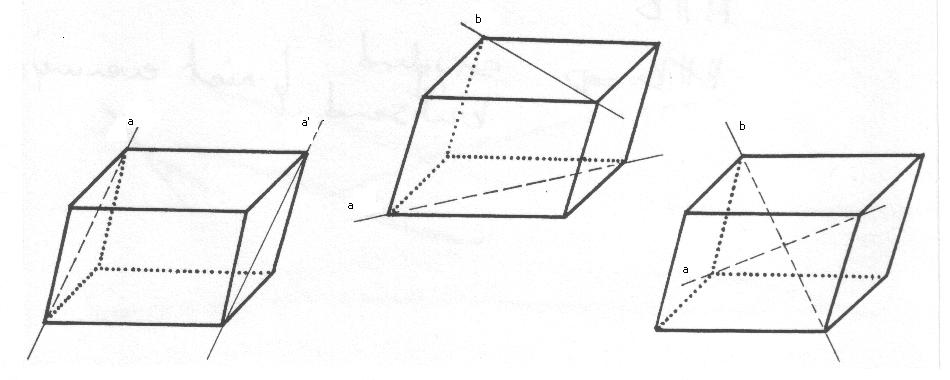
\includegraphics[width=\textwidth]{onderlinge_ligging_twee_rechten}
\end{center}

Omdat door twee verschillende punten precies één rechte gaat volgt dat twee rechten samenvallen als ze meer dan één punt gemeen hebben. Dus twee rechten $a$ en $b$ hebben
\begin{itemize}
  \item ofwel geen enkel punt gemeen:
  \begin{itemize}
    \item De rechten $a$ en $b$ hebben geen enkel punt gemeen en liggen in eenzelfde vlak. We noemen dit {\bf strikt parallelle rechten}.\\
    Notatie: $a \overset{strikt}{\parallel} b$
    \item De rechten $a$ en $b$ hebben geen enkel punt gemeen en liggen niet in eenzelfde vlak. We noemen dit {\bf kruisende rechten}.\\
    Notatie: $a\nparallel b \wedge  a \cap b = \emptyset$
  \end{itemize}
  \item ofwel juist één punt gemeen,
  \begin{itemize}
    \item De rechten $a$ en $b$ hebben juist één punt $S$ gemeen. We noemen dit {\bf snijdende rechten}. We noemen $S$ het {\bf snijpunt} van $a$ en $b$.\\
    Notatie: $a \cap b = S$
  \end{itemize}
  \item ofwel oneindig veel punten gemeen.
  \begin{itemize}
    \item De rechten $a$ en $b$ hebben alle punten gemeen. We noemen dit {\bf samenvallende rechten}.\\
    Notatie: $a = b$
  \end{itemize}
\end{itemize}

Twee rechten $a$ en $b$ zijn {\bf parallel} als ze strikt parallel zijn of samenvallend zijn.\\

\paragraph*{Stelling}
Een vlak is éénduidig bepaald door
\begin{itemize}
  \item drie niet collineaire punten.\\
  Notatie: $\vl(A,B,C)$
  \item twee strikt parallelle rechten.\\
  Notatie: $\vl(a,b)$
  \item twee snijdende rechten.\\
  Notatie: $\vl(a,b)$
  \item een rechte en een punt niet op de rechte gelegen.\\
  Notatie: $\vl(a,B)$
\end{itemize}

\end{theorie}

\begin{oefening}
\begin{enumerate}[(a)]
  \item Hoe noemen we drie punten op eenzelfde rechten?
  \item Hoe noemen we vier punten in eenzelfde vlak?
\end{enumerate}
\end{oefening}

\begin{oefening}
Wat kan je besluiten over de rechten $b$ en $c$ als de rechten $a$, $b$ en $c$ coplanair zijn, de rechten $a$ en $b$ parallel zijn en de rechten $c$ de rechte $a$ snijdt? Maak een schets.
\end{oefening}

\begin{oefening} {\em Groepswerk}\\
Zijn volgende uitspraken {\em altijd, soms of nooit} waar? Geef telkens de reden.
\begin{enumerate}[(a)]
  \item Door 4 verschillende punten gaat juist één vlak.
  \item Als twee rechten elkaar niet snijden dan liggen ze in eenzelfde vlak.
  \item Twee parallelle rechten bepalen een vlak.
  \item Als een rechte één van twee evenwijdige rechten snijdt, dan snijdt ze de andere.
  \item Door een rechte gaat minstens één vlak.
  \item Door een rechte gaan oneindig veel vlakken.
  \item Door twee verschillende rechten gaat juist één vlak.
\end{enumerate}
\end{oefening}

\begin{theorie}

\subsection{Onderlinge ligging van een rechte en een vlak}

\begin{center}
  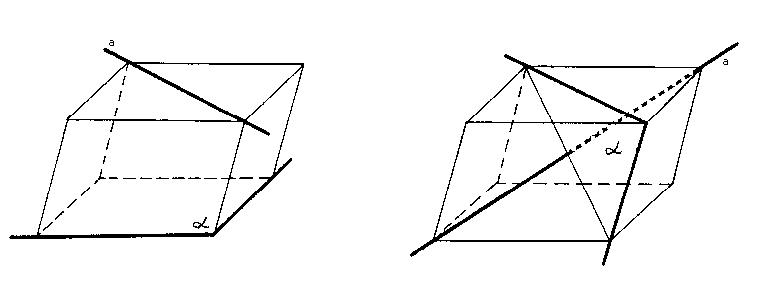
\includegraphics[width=\textwidth]{onderlinge_ligging_rechte_vlak}
\end{center}

Uit het axioma dat als twee verschillende punten van een rechte tot een vlak behoren, dat dan die rechte in dat vlak ligt volgt dat een rechte in een vlak ligt als ze met het vlak meer dan één punt gemeen heeft. Dus een rechte $a$ en een vlak $\beta$ hebben
\begin{itemize}
  \item ofwel geen enkel punt gemeen:
  \begin{itemize}
    \item We zeggen dat de rechte $a$ {\bf strikt parallel} is met een vlak $\beta$ als de rechte en het vlak geen enkel punt gemeen hebben.\\
    Notatie: $a \overset{strikt}{\parallel} \beta$
  \end{itemize}
  \item ofwel juist één punt gemeen:
  \begin{itemize}
    \item We zeggen dat de rechte $a$ {\bf snijdt} het vlak $\beta$ in het {\bf snijpunt} $S$.\\
    Notatie: $a\cap \beta = S$ 
  \end{itemize}
  \item ofwel oneindig veel punten gemeen:
  \begin{itemize}
    \item Alle punten van de rechte $a$ zijn ook punten van het vlak $\beta$. We zeggen dat de rechte $a$ in het vlak $\beta$ ligt.\\
    Notatie: $a\subset\beta$
  \end{itemize}
\end{itemize}

Een rechte $a$ is {\bf parallel} met een vlak $\beta$ als ze strikt parallel zijn of als de rechte in het vlak ligt.

\paragraph*{Stelling}
Als een rechte evenwijdig is met een vlak en een punt gemeen heeft met dat vlak dan ligt ze in dat vlak.

\paragraph*{Stelling}
Een rechte is parallel met een vlak als en slechts als de rechte parallel is met ten minste één rechte van het vlak.
\begin{center}
  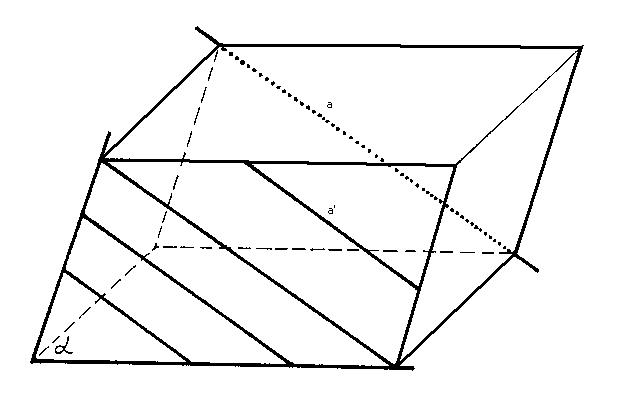
\includegraphics[width=.5\textwidth]{stelling_3}
\end{center}

\paragraph*{Stelling}
Snijdt één van twee evenwijdige rechten een vlak dan snijdt de andere ook het vlak.
\begin{center}
  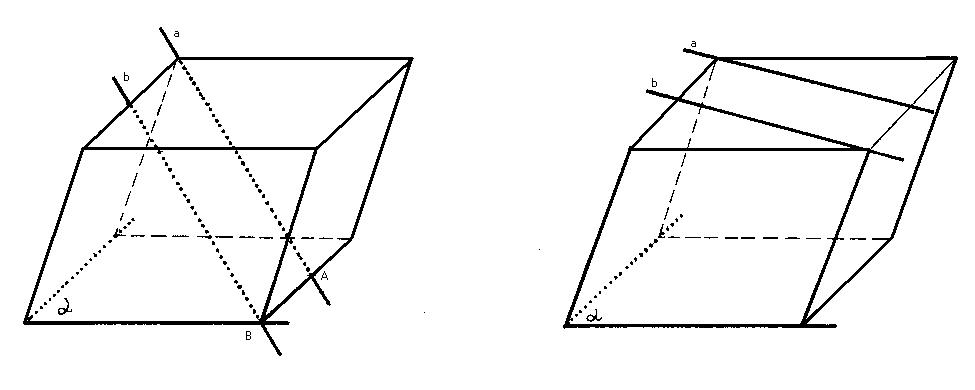
\includegraphics[width=\textwidth]{stelling_4}
\end{center}


\paragraph*{Stelling}
Als twee rechten evenwijdig zijn met eenzelfde rechte dan zijn ze onderling evenwijdig.

\paragraph*{Stelling}*
Parallellisme van rechten is een equivalentierelatie in de verzameling van de rechten van E.

\end{theorie}

\begin{oefening} {\em Groepswerk}\\
Zijn volgende uitspraken {\em altijd, soms of nooit} waar? Geef telkens de reden.
\begin{enumerate}[(a)]
  \item Als drie verschillende rechten concurrent zijn, dan liggen ze in eenzelfde vlak.
  \item Als een rechte evenwijdig is met een vlak dan is ze evenwijdig met elke rechte van dat vlak.
  \item Als twee rechten evenwijdig zijn met eenzelfde vlak dan zijn ze onderling evenwijdig.
  \item Een rechte evenwijdig met de snijlijn van twee vlakken is evenwijdig met beide vlakken.
\end{enumerate}
\end{oefening}

\begin{theorie}

\subsection{Onderlinge ligging van twee vlakken}

\begin{center}
  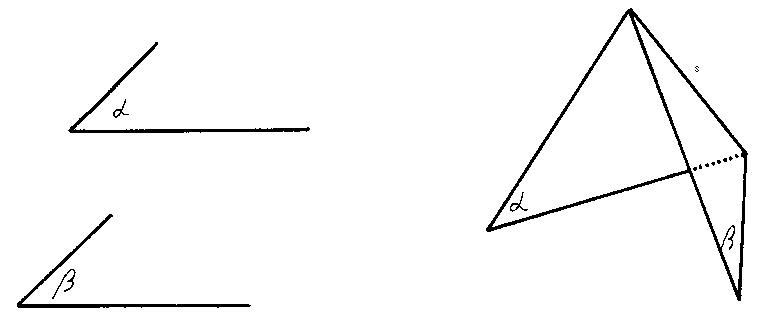
\includegraphics[width=.7\textwidth]{onderlinge_ligging_twee_vlakken}
\end{center}

Voor twee vlakken $\alpha$ en $\beta$ doet zich één van de volgde mogelijkheden voor
\begin{itemize}
  \item Hebben twee vlakken $\alpha$ en $\beta$ geen enkel punt gemeen dan noemen we ze {\bf strikt parallel}.\\
  Notatie: $\alpha \overset{strikt}{\parallel}\beta$
  \item Hebben twee verschillende vlakken $\alpha$ en $\beta$ ten minste één punt gemeen dan hebben ze een rechte door dat punt gemeen. We noemen $\alpha$ en $\beta$ dan {\bf snijdende vlakken} met de {\bf snijlijn} s.\\
  Notatie: $\alpha \cap \beta = s$
  \item Hebben twee vlakken tenminste drie niet-collineaire punten gemeen dan vallen ze samen en noemen we ze {\bf samenvallende vlakken}.
\end{itemize}

Twee vlakken $\alpha$ en $\beta$ zijn {\bf parallel} als ze strikt parallel of samenvallend zijn.

Opmerking: In de ruimte kunnen we een rechte bepalen door:
\begin{itemize}
  \item twee verschillende punten,
  \item twee snijdende vlakken.
\end{itemize}

\paragraph*{Stelling}
Is een rechte parallel met elk van twee snijdende vlakken dan is ze parallel met de snijlijn van de twee vlakken.
\begin{center}
  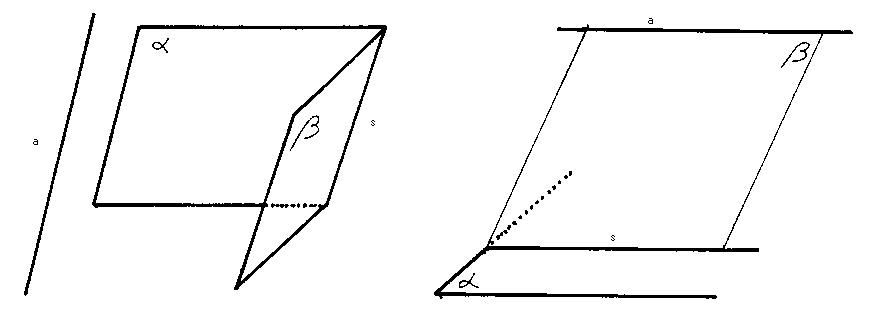
\includegraphics[width=.7\textwidth]{stelling_8}
\end{center}

\paragraph*{Stelling}
Zijn twee vlakken parallel, dan is elke rechte van het ene vlak parallel met het andere vlak.

\paragraph*{Stelling}
Twee vlakken zijn parallel als twee snijdende rechten van het ene vlak parallel zijn met resp. twee rechten van het tweede vlak.

\paragraph*{Stelling}
\begin{itemize}
  \item Snijdt een rechte één van twee parallelle vlakken dan snijdt ze ook het andere vlak.
  \item Is een rechte parallel met één van twee parallelle vlakken dan is ze ook parallel met het andere vlak.
  \item Snijdt een vlak één van twee evenwijdige vlakken dan snijdt ze ook het andere, en de snijlijnen zijn evenwijdig.
\end{itemize}
\begin{center}
  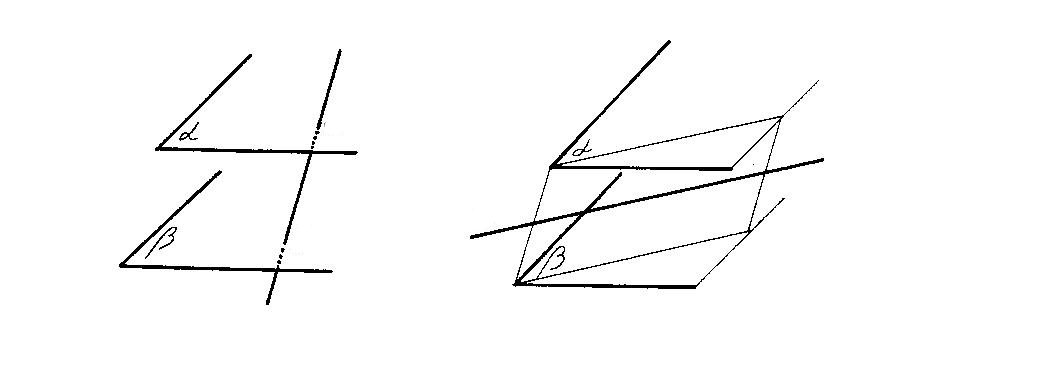
\includegraphics[width=.7\textwidth]{stelling_11}
\end{center}

\paragraph*{Stelling}
Als twee vlakken parallel zijn met eenzelfde vlak dan zijn ze onderling parallel.

\paragraph*{Stelling}
Door elk punt gaat juist één vlak parallel met een gegeven vlak.

\paragraph*{Stelling}*
Parallellisme van vlakken is een equivalentierelatie in de verzameling van de vlakken van E.

\paragraph*{Stelling}
Door elk punt gaan oneindig veel rechten parallel met een gegeven vlak.
Deze rechten vormen een stralenbundel met top het gegeven punt en liggen allemaal in een
vlak evenwijdig met het gegeven vlak.
\begin{center}
  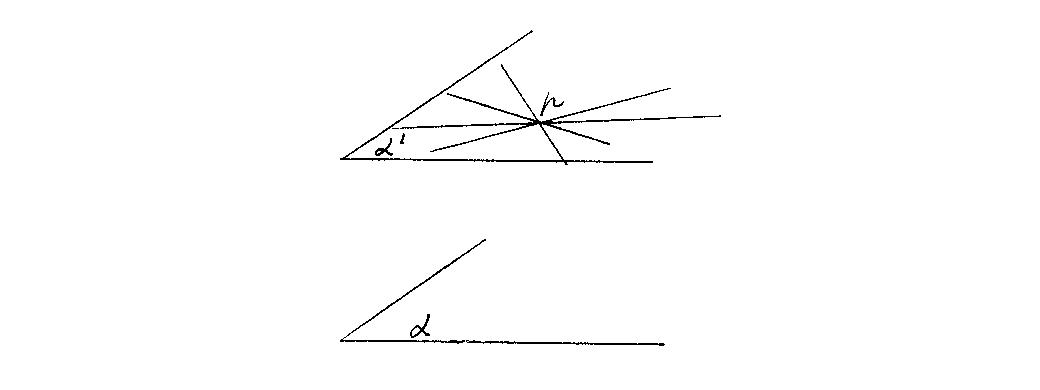
\includegraphics[width=\textwidth]{stelling_17}
\end{center}
\end{theorie}

\begin{oefening}
De snijpunten van twee strikt parallelle rechten en twee strikt parallelle vlakken zijn
de hoekpunten van een parallellogram. Welke vlakke figuur krijgen we als we twee
snijdende rechten snijden met twee strikt parallelle vlakken? Maak een schets voor
elk van de 3 mogelijkheden.
\end{oefening}

\begin{oefening} {\em Groepswerk}\\
Zijn volgende uitspraken {\em altijd, soms of nooit} waar? Geef telkens de reden.
\begin{enumerate}[(a)]
  \item Als twee vlakken niet parallel zijn dan zijn ze snijdend.
  \item Als één van twee snijdende rechten parallel is met een vlak dan is de andere rechte parallel met dat vlak.
  \item Twee vlakken zijn evenwijdig als twee snijdende rechten van het ene vlak evenwijdig zijn met het andere vlak.
  \item Een vlak evenwijdig met de snijlijn van twee vlakken is evenwijdig met beide vlakken.
  \item Door een rechte gaat één vlak parallel met een gegeven vlak.
  \item Door elk van twee kruisende rechten kunnen we een vlak aan brengen, zó dat beide vlakken parallel zijn.
  \item Als twee vlakken evenwijdig zijn en men door een punt van het eerste vlak een rechte trekt parallel met het tweede vlak dan ligt die rechte in het eerste vlak.
  \item Door een punt gaat juist één rechte parallel met een gegeven vlak.
  \item Als twee vlakken evenwijdig zijn met eenzelfde rechte dan zijn ze onderling evenwijdig.
\end{enumerate}
\end{oefening}

\begin{oefening}
{\em Gegeven:} twee parallelle vlakken $\alpha$ en $\beta$ , twee punten $A$ en $B$ van $\beta$ , een punt $C$
van $\alpha$, een rechte $l$ van $\alpha$, de rechte $m$ door $B$ parallel met $AC$.\\
{\em Construeer:}
\begin{enumerate}[(a)]
  \item het snijpunt van $\alpha$ en $m$;
  \item het snijpunt van $\vl(A, B, C)$ en $l$.
\end{enumerate}
\end{oefening}

\begin{oefening}
{\em Gegeven:} twee snijdende vlakken $\alpha$ en $\beta$ en hun snijlijn $s$, twee punten $A$ en $B$ van $\alpha$.\\
{\em Construeer:} het snijpunt van $AB$ en $\beta$.
\end{oefening}

\begin{oefening}
Construeer een rechte die door een gegeven punt gaat, een gegeven rechte snijdt en
evenwijdig is met een gegeven vlak.
\end{oefening}

\begin{theorie}

\pagebreak
\section{Begrip coördinaat}

\subsection{Assenstelsel}

Kiezen we in onze ruimte $E^3$ een oorsprong $\vec{o}$ en drie niet-nul vectoren $\vec{e}_1$, $\vec{e}_2$ en $\vec{e}_3$ die niet samen met $\vec{o}$ in eenzelfde vlak liggen, dan bepaalt dit drietal $(\vec{e}_1, \vec{e}_2, \vec{e}_3)$ een {\bf basis} in $E^3$. We ijken de assen door de oorsprong $\vec{o}$ met het getal $0$ te laten overeenkomen en door elke van de vectoren $\vec{e}_1$, $\vec{e}_2$ en $\vec{e}_3$ met het getal $1$ te laten overeenkomen. We noemen nu nog de rechte door $\vec{o}$ en $\vec{e}_1$ de $x$-as, de rechte door $\vec{o}$ en $\vec{e}_2$ de $y$-as en de rechte door $\vec{o}$ en $\vec{e}_3$ de $z$-as. Op deze manier krijgen we een willekeurig assenstelsel wat we een {\bf affien assenstelsel} noemen horende bij een {\bf affiene ruimte}. We eisen nu nog dat de drie assen $x$, $y$ en $z$-as twee aan twee loodrecht op elkaar liggen. Op deze manier krijgen we ons {\bf orthonormaal assenstelsel} horende bij de {\bf euclidische ruimte}.

We kunnen zo een orthonormaal assenstelsel eenvoudig voorstellen m.b.v. een kubus.

\subsection{Coördinaten}

Als we in $E^3$ een basis $(\vec{e}_1, \vec{e}_2, \vec{e}_3)$ hebben, dan kan elk punt $\vec{a}\in E^3$ met $a_1, a_2, a_3 \in \mathbb{R}$ op een unieke manier geschreven worden als
$$\vec{a} = a_1\vec{e}_1 + a_2\vec{e}_2 + a_3\vec{e}_3$$

Het drietal $(a_1, a_2, a_3)$ bepaalt dus eenduidig het punt $\vec{a}$. We noemen $(a_1, a_2, a_3)$ de {\bf coördinaat} van $\vec{a}$ t.o.v. de basis $(\vec{e}_1, \vec{e}_2, \vec{e}_3)$. We kunnen dus voor het punt $\vec{a}$ kort schrijven $\vec{a}=(a_1, a_2, a_3)$ of in matrixnotatie:
$$\vec{a}=\begin{pmatrix}a_1\\a_2\\a_3\end{pmatrix}$$

In wat volgt veronderstellen we dat een oorsprong en een basis gekozen zijn zodat we ons orthonormaal assenstelsel horende bij de euclidische ruimte krijgen.

\pagebreak
\section{Bewerkingen met coördinaten}

\pagebreak
\section{Zwaartepunt van 2, 3 of 4 onafhankelijke punten}

\pagebreak
\section{Rechten}

\pagebreak
\section{Vlakken}

\pagebreak
\section{Afstand, norm en inproduct}

\pagebreak
\section{Onderlinge ligging van rechten en vlakken}

\pagebreak
\section{Afstand tussen punten, rechten en vlakken}

\end{theorie}

\end{document}

